% !TEX root = ../main.tex

\chapter{Reinforcement learning basics}
\label{ch:reinforcement_learning}

\section{Reinforcement learning and continuous control}

\subsection{Reinforcement learning paradigm}
A learning paradigm is a formal description of a framework that enables the learning process by defining the sources of information to learn from, establishing criteria for assessing the effectiveness of a learning solution, and identifying the available resources that can enhance the learning process. Essentially, a learning paradigm provides a formal description of the underlying principles and assumptions that guide how we learn and improve our knowledge and skills.

The paradigm involves the interaction between two main components: an agent and an environment. The environment represents the "world" in which the agent operates and provides information about its current state. The agent, on the other hand, is responsible for taking actions within the environment. It acts on the environment by performing available actions and controls, perceives and assesses the changes occurring in the environment via the senses at its disposal, and engages in a feedback loop that informs and modifies its future behavior. Each interaction between the agent and the environment follows a sequence: the agent receives observations based on the current state of the environment, selects an action to take, and transmits that action to the environment. In response, the environment updates its internal state and provides feedback to the agent in the form of updated observations and a reward signal. The reward signal indicates the success or suitability of the agent's action in completing a task, while the updated observations provide information about the new state of the environment. The reward function, also called the fitness, is the only signal required for this learning method to improve and estimate how good a solution is. Figure~\ref{fig:RL_main_loop} depicts a single timestep of interaction between the agent and the environment.

Reinforcement learning is different from other machine learning approaches such as supervised learning, which uses labeled data to predict outputs for unseen data, and unsupervised learning, which seeks to find patterns in unlabeled data. Reinforcement learning is both a problem that can be addressed with specific solution methods and a field of study that examines the problem and its potential solutions. Unlike supervised learning, there are no labeled data available in reinforcement learning, so the agent learns by maximizing its performance based on the reward signal (\cite{sutton_reinforcement_1998})

\subsection{Continuous control}
A control problem involves a dynamic system described by state variables, and the goal is to determine a strategy that leads the system to its desired target state. The agent, which takes actions and is part of the environment, sends actions to determine the future behavior of the system. In continuous control problems, the system is observable at all times, and there is continuous interaction between the agent and the environment. An example is self-driving cars, which require continuous adaptation of behavior to drive optimally. To simplify the analysis of dynamic systems, time is often discretized into time-steps. This approach provides a way to break down the system's behavior into manageable intervals that can be analyzed and optimized. However, in practice, the accuracy of the analysis is often limited by the control frequency, which is the rate at which the system's inputs can be adjusted. If the control frequency is sufficiently high, the discretization of time becomes less critical, as the system's behavior can be accurately captured by the rate at which the inputs are adjusted. Therefore, the use of time-steps provides a useful tool for simplifying the analysis of dynamic systems, but the accuracy of the analysis ultimately depends on the system's control frequency (\cite{franklin_feedback_2014}).

Both continuous control and reinforcement learning aim to design systems with richly structured perception, perform planning and control that adapt effectively to environmental changes, and exploit safeguards in the face of new scenarios (\cite{recht_tour_2018}).


\section{Classical reinforcement learning}

Some challenges cannot be solved through traditional problem-solving methods or supervised learning algorithms, and reinforcement learning is necessary to tackle them effectively. 
The Classical Reinforcement Learning framework is a comprehensive system designed with the sole purpose of enabling optimal interactions between agents and their environment. The framework is founded on the principle of trial-and-error learning, where the agent learns through experience by interacting with the environment, and receiving feedback in the form of rewards or penalties. The framework is structured to optimize the agent's behavior, allowing it to learn the best actions to take in any given situation. This broad framework is applicable across a range of contexts, and it has been successfully employed in various fields such as robotics, game-playing, and autonomous vehicles, among others.

\begin{figure}[!ht]
\centering
\fbox{\includegraphics[width=.7\textwidth]{RL_main_loop}}
\caption[Main interaction of the agent and the environment in reinforcement learning]{
  \textbf{Main interaction of the agent and the environment in reinforcement learning.}
  At the beginning (timestep $t$) the agent gets the observation $S_t$ and the reward $R_t$ from the environment. The agent performs then action $A_t$ and sends it to the environment. The environment changes its state and returns a new observation $S_{t+1}$ and a new reward $R_{t+1}$.
 }
\label{fig:RL_main_loop}
\end{figure}


In reinforcement learning, the policy is a key element of the framework that determines the actions an agent should take in different states of the environment. The policy is represented by a mapping from states to actions, and it can be either deterministic or stochastic. Deterministic policies specify a single action to take in each state, while stochastic policies specify probabilities for different actions to occur. The reward an agent receives depends on the chosen policy, and the sequence of states reached by the agent is called a Markov chain. In the Classical Reinforcement Learning framework, all reinformcement learning algorithms describe the problem as a Markov chain, which captures the essential properties of the agent's environment. This mathematical concept models systems that change over time in a way that depends only on the current state and not on the history of past states(\cite{sutton_reinforcement_2018}). The algorithms then analyze the interactions between the agent and its environment, focusing on observations, actions, and rewards. The rewards are often modeled to simplify the policy, which is the strategy that the agent uses to decide on its actions based on the current state of the environment. The modeling of rewards can be done using various techniques, including value function or q-function, among others.


The value function is a key concept in reinforcement learning that allows us to evaluate the effectiveness of different policies.$V_{\pi}(s)$ defines the expected total reward that an agent can expect to receive by following the policy $\pi$, starting from state $s$. One way to compute the value function is using the Bellman equation (\ref{bellman}),
\begin{equation}\label{bellman}
V_{\pi}(s) = R(s, \pi(s)) + \gamma \sum_{s' \in S} P_{s, s'}^{\pi(s)} V_{\pi}(s')
\end{equation}
which expresses the value of a state in terms of the values of its successors(\cite{barron_bellman_1989}). $R(s, \pi(s))$ describes the reward obtained by doing the action chosen by $\pi(s)$ in state $s$.$\gamma$ enables to give more or less importance to the rewards that occur later. $ P_{s, s'}^{\pi(s)}$ describes the probability of reaching $s'$, after executing the action chosen by $\pi(s)$ in the state $s$ and $V_{\pi}(s')$ stands for the future reward collected by the agent following policy $\pi$ starting from the state $s'$. It is also important to note, the Bellman equation does not have a closed-form solution, which makes it challenging to compute the value function in practice.
The value function can be used to define an optimal policy, which is the policy that is expected to maximize the reward over time. Another way to analyze policies is using the Q-function.$Q_{\pi}(s, a)$ is defined as the expected total reward acquired by the agent following policy $\pi$ starting from state $s$ and taking action $a$. The Q-function can be related to the value function through the equation $V_{\pi}(s) = Q_{\pi}(s, \pi(s))$. A common method for finding the optimal Q-function is Q-learning, which is an iterative process that updates the Q-function based on experience (\cite{watkins_q-learning_1992}). 


Reinforcement learning is well-suited for autonomous systems that learn to achieve a desired outcome through trial and error. However, this paradigm presents a unique challenge that is not encountered in supervised or unsupervised learning: balancing exploitation and exploration. Exploitation refers to the process of repeating actions that have resulted in positive rewards in the past, in order to maximize the cumulative reward. On the other hand, exploration involves trying new actions in order to potentially discover higher rewards and avoid getting stuck in a local optimum. Finding the right balance between these two approaches is crucial for the success of the learning process. There are a lot of strategies for this including $\epsilon - greedy$ selection and $Q-learning$, but still a lot of research is done to find more effective solutions (\cite{coggan_exploration_nodate}).

Reinforcement learning has been effective in solving a range of tasks, ranging from simple games to complex real-world problems in fields such as robotics, games and autonomous driving. However, it has also encountered challenges in these real-world applications (\cite{zhu_ingredients_2020}). Nevertheless, the paradigm is sufficient for addressing the desired tasks in this thesis.

In conclusion, reinforcement learning offers a powerful tool for training agents to make decisions in dynamic environments and optimize for a given reward signal. It can effectively solve a range of problems while also presenting the unique challenge of balancing exploitation and exploration.

\section{Direct Policy Search}
Direct policy search is a method for solving reinforcement learning problems. It is a type of policy search algorithm that aims to directly optimize the policy, as opposed to value-based methods which use a value function approximation.

One of the primary benefits of direct policy search is its ability to handle high-dimensional and continuous action spaces, making it well-suited for problems with complex and continuous control tasks, such as robotics and autonomous systems.

To improve performance and better understand how network complexity contributes to representing the policy, the network in direct policy search can be separated into two components: one for learning intermediate representations of the input, and another for learning the policy (\cite{cuccu_playing_2019}). This separation enables the use of smaller networks dedicated to policy learning.

Direct policy search can be implemented using various techniques, including gradient-based optimization methods and evolutionary algorithms. The choice of method depends on the specific problem and constraints and may involve trade-offs between computational efficiency and solution quality.

\section{Neuroevolution}

Neuroevolution  is a technique that leverages black-box optimization, usually evolutionary algorithms, to determine the parameters of a neural network. The fitness function assesses the network by transforming the individual into weight matrices and inserting them into the network. Neuroevolution brings both the advantages and drawbacks of evolutionary algorithms to the challenge of finding a suitable neural network model.

In reinforcement learning, neuroevolution can be utilized for direct policy search, eliminating the need for supervised learning. The only necessary information is the reward function, not labeled actions. While neuroevolution for direct policy search in reinforcement learning has its advantages, there are also some limitations to consider. Firstly, these algorithms are computationally expensive and may not be as efficient as gradient-based algorithms. Additionally, since the performance of randomized algorithms depends on random events such as mutations, their performance can vary significantly across runs and there are no guarantees. Furthermore, neuroevolution algorithms only use the cumulative reward at the end of an episode and miss the correspondence between individual actions and per-step rewards.

For this project, the same concept is applied but using binary trees instead of neural networks. A proposal for the name of this method is "Treeevolution".

\section{Black-Box Optmization}

In mathematics, optimization refers to the process of finding the maximum or minimum value of an objective function. Neural networks, for example, try to find the best weights for approximating an underlying function using techniques such as backpropagation and gradient descent. However, these techniques require knowledge of the derivative of the function, which may not always be available or may be too complex to compute (\cite{schaul_studies_nodate}). Black-box optimization is a method that does not rely on any assumptions about the function or its properties, and can be used to optimize any function approximator. It is based on a feedback score similar to reinforcement learning, and the parameter set is improved based on this score (\cite{anderson_introduction_1995}).

Black-box optimization methods are generally less efficient than traditional techniques such as gradient descent because they do not take advantage of information about the structure of the function being optimized. This means they must explore a larger space of possible solutions, which can be time-consuming. However, black-box optimization methods can be effective in situations where the function being optimized is highly complex or has a large number of variables, and traditional methods may not be applicable. They are also flexible and can be applied to a wide range of problems without requiring any knowledge of the function being optimized.

In optimization problems, techniques typically converge to a single optimum, which is referred to as unimodality. On the other hand, multimodality refers to the presence of multiple distinct optima in the objective function, which is more common in real-world applications. Solving multimodal problems requires exploration in addition to the exploitation used in single-optimum problems. For example, gradient descent only uses exploitation and can only find another local optimum through exploration by restarting with a different initialization.

Black-box optimization methods, which do not depend heavily on knowledge of the function, can be well-suited for handling multimodal problems because they can explore a larger space of possible solutions. However, one challenge in multimodal landscapes is avoiding getting stuck in a local optimum before reaching the global optimum. A solution to this challenge is to generate multiple viable parametrizations, each exploring a different area in the optimization space. This technique gives a better understanding of the landscape and provides direction for where the most improvement can be obtained. An example of a method for generating parametrizations with improving scores is evolutionary algorithms.

\subsection{Random weight guessing}
The simplest version of an optimizer is to randomly select the set of weights, also known as random initialization, and keep always the best performing individuals. Algorithm \ref{algo:random_weight_guessing} shows this procedure. This procedure is called random weight guessing. By randomly initializing the weights, the network is able to explore a wide range of possible solutions, increasing the chances of finding a good global minimum. Even with its simple implementation, random weight guessing has shown some great results in Classic Control benchmarks from the OpenAI Gym (\cite{oller_analyzing_2020}). It's important to note that the initialization of the weights can have a significant impact on the performance of the neural network. Thus, the chosen range for the randomly selected weights will have an impact on the result. Choosing a suitable range for the randomly selected weights is important to ensure that the network can learn useful features and avoid getting stuck in a poor local minimum during the training process. However, it should be noted that random weight guessing will have some limitations with complex problems due to the large search space, because of the large number of possible weight combinations, which can make it difficult for the algorithm to find the global optimum.

\begin{algorithm}
\caption{\texttt{random weight guessing} algorithm}
\label{algo:random_weight_guessing}
\begin{algorithmic}[1]
\State $best\_ind \gets None$ \Comment No best performing individual at the beginning
\State $best\_fit \gets -inf$ \Comment fitness of best performing individual
\While {stopping criterion not reached}
  \State generate a population randomly
  \State evaluate fitness of each $individual$ 
  \If {fitness of $individual$ > $best\_fit$}
    \State $best\_ind \gets individual$
    \State $best\_fit \gets fitness of individual$
  \EndIf
\EndWhile
\end{algorithmic}
\end{algorithm}


\subsection{Evolution strategies}

Evolution strategies (ES) is a class of evolutionary algorithms that is specialized for optimization of continuous variables. Inspired by natural evolution, ES is a black-box optimization algorithm that uses a process of mutation and selection to search for good solutions to a given problem. In the main loop of the algorithm, new individuals are created by mutating the parent individuals of the current generation. An individual in the context of ES refers to a specific set of parameters being optimized by the algorithm. A population is a group of individuals being considered by the algorithm at a given time, and a generation refers to one iteration of the main loop. The fitness of an individual is a measure of its performance or quality, based on the feedback score provided by the algorithm.

The main loop of the ES algorithm consists of creating new individuals from the parent individuals of the current generation, evaluating their fitness, and selecting the best-performing individuals to be the parent individuals for the next generation. This process continues until a sufficient solution is found, as determined by a stopping criterion. Algorithms differ in the number of offsprings created per generation, the number of selected individuals for the next generation, and how the mutation process is performed. Other than gradient-descent based methods, ES generates multiple individuals and by that explores different areas or paths of the optimization space independently, which can be beneficial for avoiding local optima and solving real-world problems that may require sophisticated exploration mechanisms. It is important to note that the efficiency of Evolution Strategies highly depends on factors like the population size, or the mutation and selection methods used. To maximize their performance, experimenting on this factors with different configuration setting might be useful(\cite{salimans_evolution_2017}). 


\subsection{Covariance Matrix Adapation Evolution Strategy}
CMA-ES (Covariance Matrix Adaptation Evolution Strategy) is a stochastic optimization algorithm that is used to optimize complex non-linear functions. It is a derivative-free optimization method that is particularly well-suited for high-dimensional problems. The algorithm works by maintaining a distribution of candidate solutions (i.e. a population of possible solutions) and adapts the distribution based on the performance of the solutions. It is based on the evolution strategy algorithm and uses a covariance matrix to adapt the distribution. The algorithm iteratively updates the distribution until it converges to a solution that is close to the global optimum (\cite{akimoto_theoretical_2012}).

The algorithm has several hyperparameters that can be adjusted to optimize its performance and highly influence its efficiency. Some of the most important ones include: population size, step size (represented by "sigma" parameter), number of generations, number of parents (represented by "mu" parameter), and so on. The "mu" parameter represents the number of solutions (or parents) that are selected from the population to generate the next generation of solutions and it determines the balance between exploration and exploitation in the search process. The "sigma" parameter represents the step size of the search, it controls the scale of the search and determines how far the algorithm moves away from the current best solution in each generation, it also adjusts the standard deviation of the multivariate normal distribution that guides the search. CMA-ES is a robust optimization algorithm that is widely used. Figure \ref{fig:cma_es} illustrates the evolution of the search distribution for CMA-ES on a simple quadratic function, which is a minimization task. The function is defined as $(x - 5) ^ 2 + (y - 5) ^ 2$. The background of the plot indicates good solutions with dark red colors and less good solutions with lighter colors. The red cross represents the optimal solution at coordinates $(5,5)$. The CMA-ES algorithm starts with a standard deviation of one and an initial population initialized with zeros. In the early stages of the optimization process, the search distribution will grow, leading to a high level of exploration. The search distribution is represented by a yellow ellipse, where the center of the ellipse is the mean of the current solutions and the width and height of the ellipse are twice the standard deviation of the search distribution. As the optimization progresses, the search distribution becomes more focused on finding the best individuals and converging towards the global optimum.

\begin{figure}[!ht]
\centering
\fbox{\includegraphics[width=0.8\textwidth]{cma_evolution_search_distr}}
\caption[Optimization of a 2D problem with CMA-ES]{
  \textbf{Optimization of a 2D problem with CMA-ES}
  Illustration of a population reaching the global optimum in twelve generations. The background displays the fitness landscape, with red colors indicating higher scores. The red cross indicates the optimal score. The population is represented by black dots, and the yellow ellipse represents the search distribution.
 }
\label{fig:cma_es}
\end{figure}

\section{Benchmarks for reinforcement leaning control problems}

A benchmark environment in the context of reinforcement learning (RL) is a standard and well-defined scenario that serves as a reference point for evaluating and comparing the performance of different RL algorithms. These environments usually provide a clear definition of the state space, action space, reward structure, and other problem specifications. By using common benchmark environments, researchers and practitioners can easily compare the performance of their algorithms to those of others, and determine which algorithms are best suited for specific types of RL problems. A commun benchmark environment is OpenAI Gym, which will be used in this project.

\subsection{OpenAI Gym}

Open Ai Gym is a toolkit that provides a variety of environments for developing and comparing reinforcement learning algorithms. One of its main advantages is that is uses the same interface for every task which enables an easy comparison and reproduction of results. It offers a range of environments for training agents, including classical control problems, Atari games, and physics simulations which vary in difficulty. OpenAI Gym offers tools for evaluating and visualizing the performance of the algorithms such as pre-built plotters and metrics. All of this gives big advantages for the research community in the field of reinforcement learning (\cite{noauthor_openai_2016}). There are many different categories of environments available. The less complex environments are the classical control problems and can usualy be solved rapidely. The environments used in the context of this project are of the category of Box2D environments. Those problems are harder to solve and are highly configurable. Another category are Atari games, which are a collection of classic video games from the 1980s that were released for the Atari 2600 console. These games are relatively simple by modern standards, but they are still challenging for machine learning algorithms because they require the agent to learn to make decisions in a complex and dynamic environment.

Some of the Atari games included in OpenAI Gym are Pong, Breakout, Space Invaders, and Pac-Man. These games have become popular benchmarks for reinforcement learning algorithms because they are simple enough to be used as a starting point for research, but complex enough to pose a challenge(\cite{brockman_openai_2016}). Figure~\ref{fig:atari_games} illustrates some of the Atari games available in OpenAI Gym.

\begin{figure}[!ht]
\centering
\fbox{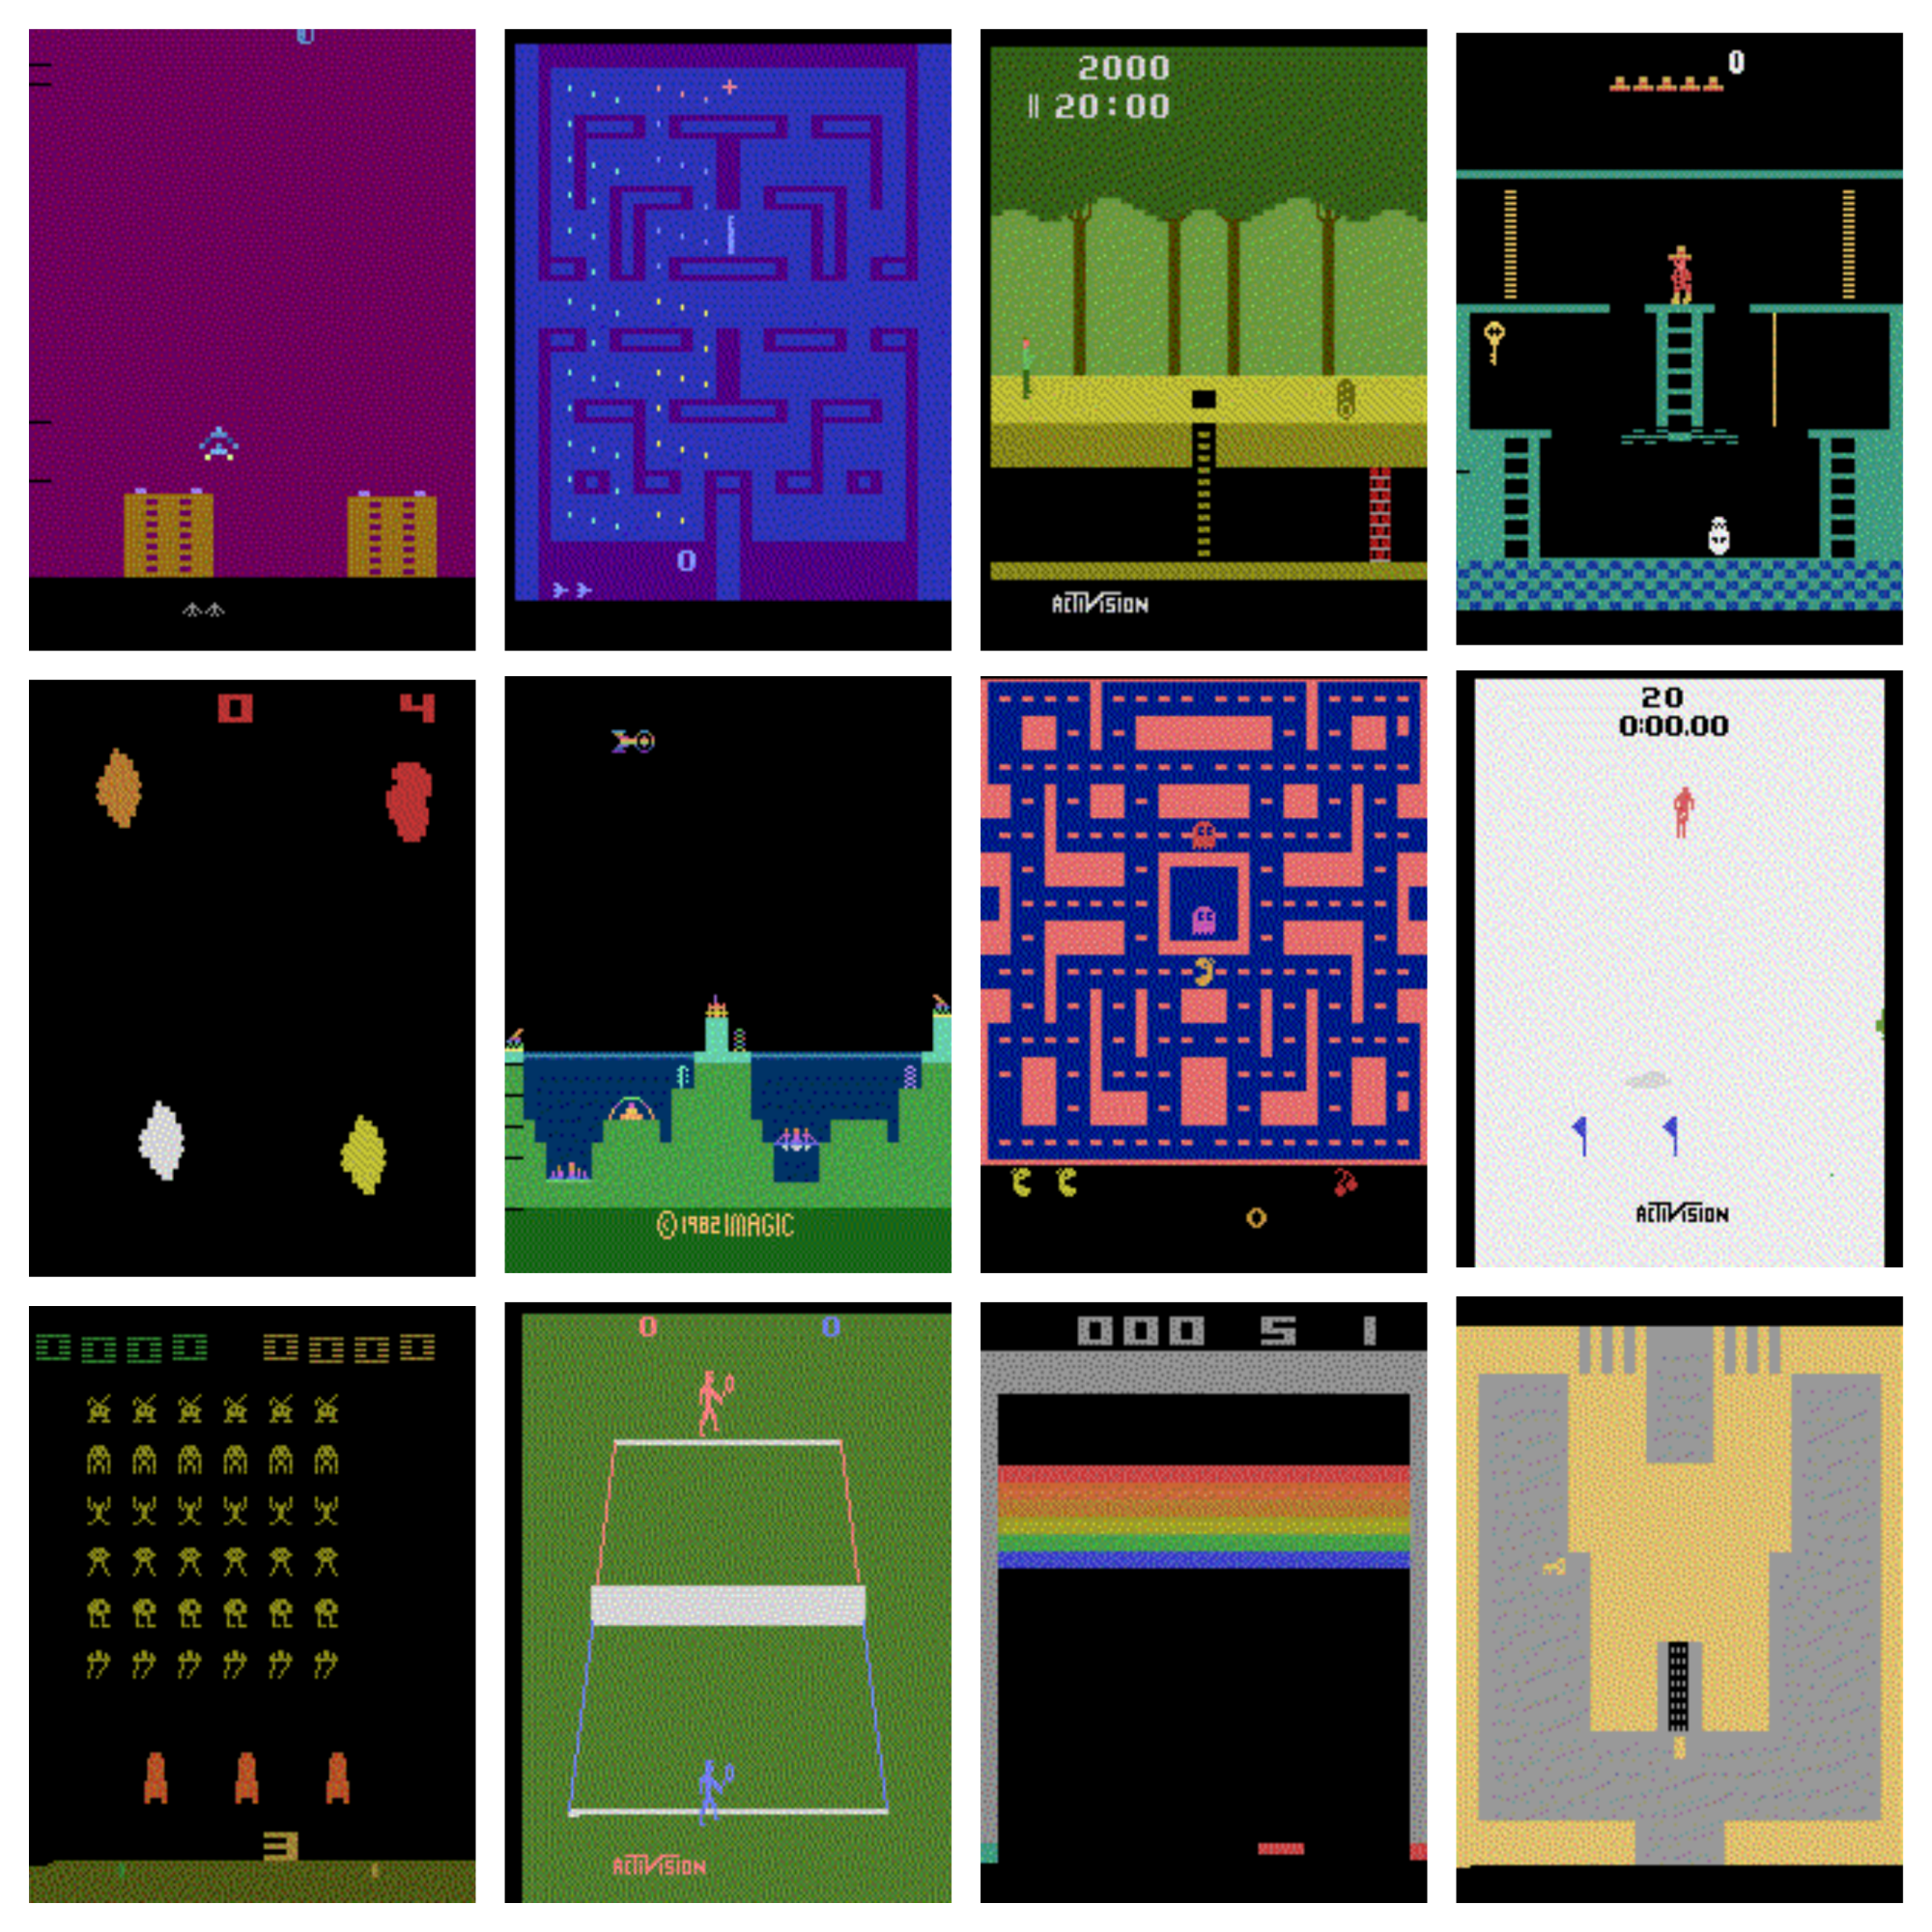
\includegraphics[width=0.8\textwidth]{atari_games}}
\caption[Atari games of OpenAI Gym]{
  \textbf{Some Atari games of OpenAI Gym}
  Illustration of a subset of the Atari environments available in OpenAI Gym. The represented environments from left to right and from the top to the bottom are: Air Raid, Alien, Pitfall, Montezuma Revenge, Asteroids, Atlantis, Ms Pacman, Skiing, Space Invaders, Breakout and Adventure
 }
\label{fig:atari_games}
\end{figure}



To start working with the toolkit, the first step is to generate an instance of a specified envrionment. This can be done with the predefined function $gym.make()$ to which we pass the name of the environment we want to generate as parameter. The environment can then be stored as a variable and can be reset to its initial state with the $reset()$ function which is typically done at the beginning of an episode and gives out the observations of the current state and some extra information. The observation is often used to get an action from a model which is then passed as argument to the predefined function $step()$. This function returns the next state, the reward obtained, a boolean indicating wheter the episode is over and some extra information too. These are just some basic functions that enable to start developing and evaluating reinforcement learning algorithms with the help of OpenAI Gym.







